\section{Context}

\Glspl{sadapt} optimize their \glspl{behaviour} or configurations at runtime in response to a modification of their \glspl{env} or their \glspl{behaviour}~\cite{DBLP:conf/dagstuhl/ChengLGIMABBBCSDFGGGKKKLMMMPSTTWW09}.
Kephart and Chess~\cite{DBLP:journals/computer/KephartC03} laid the groundwork for this approach, based on an IBM white paper~\cite{computing2006architectural}.
Since then, practitioners have applied it to different domains~\cite{DBLP:journals/corr/abs-1904-01518} such as cloud infrastructure~\cite{DBLP:conf/icac/JavadiG17, OpenStack:Watcher:Wiki, DBLP:conf/icse/BarnaKFL17} or \gls{cps}~\cite{DBLP:conf/icac/LalandaGC17, DBLP:conf/cbse/FouquetMFBPJ12, DBLP:conf/smartgridsec/0001FKNT14}.
One example of such a system is a \gls{sg}, which employs the adaptation capacity to heal itself autonomously.

A \gls{sg} is a power grid in which utilities introduce \gls{ict} to face the new challenges of electricity supply~\cite{farhangi2010path, ipakchi2009grid, DBLP:journals/comsur/FangMXY12}.
One of the required feature is the \gls{shealing} capacity.
A \gls{shealingSyst} can automatically repair any incident, software or hardware, at runtime~\cite{DBLP:journals/computer/KephartC03}.
For example, a smart grid can optimise the power flow to deal with failures of transformers\footnote{Transformers change the voltage in the cables.}~\cite{DBLP:journals/comsur/FangMXY12}.

The adaptation process can be performed only if the system has a deep understanding of the situation and the problem.
In this case, the situation comprises the \gls{structure} (elements that compose the system), the \gls{behaviour} (the set of possible \glspl{exec} of the system) and the \gls{env} (where it is executed) of the system.
This understanding can be extracted from an, or a set of, \textbf{abstraction}(s) of these elements.
Abstractions provide a description of systems, their \glspl{behaviour}, or their \glspl{env}.
For example, Hartmann~\etal \cite{DBLP:conf/smartgridcomm/0001FKTPTR14} provide a class diagram that describes the smart grid topology, when it uses power lines communications\footnote{Data are sent through cables that also distribute electricity.}.

\textbf{\Gls{mde}} defenders argue for using the abstraction mechanism to facilitate the development of current software~\cite{DBLP:journals/computer/Schmidt06, DBLP:conf/ifm/Kent02, DBLP:series/synthesis/2017Brambilla}.
This methodology can be applied to different stages of software development.
In this thesis, we focus on one of its paradigms: \textbf{\gls{m@rt}}~\cite{DBLP:journals/computer/BlairBF09, DBLP:journals/computer/MorinBJFS09}.
As we depict in \Cref{fig:intro:context:m@rt}, using this paradigm, the adaptation process relies on a \gls{model} for analysing the situation and triggering the adaptation.
In this document, we say that the model represents the knowledge of the adaptation process.
Developers can use this paradigm to implement \glspl{adptSyst}~\cite{DBLP:journals/computer/MorinBJFS09, DBLP:conf/smartgridsec/0001FKNT14}.
This dissertation contributes to this modelling layer.



\begin{figure}
	\centering
	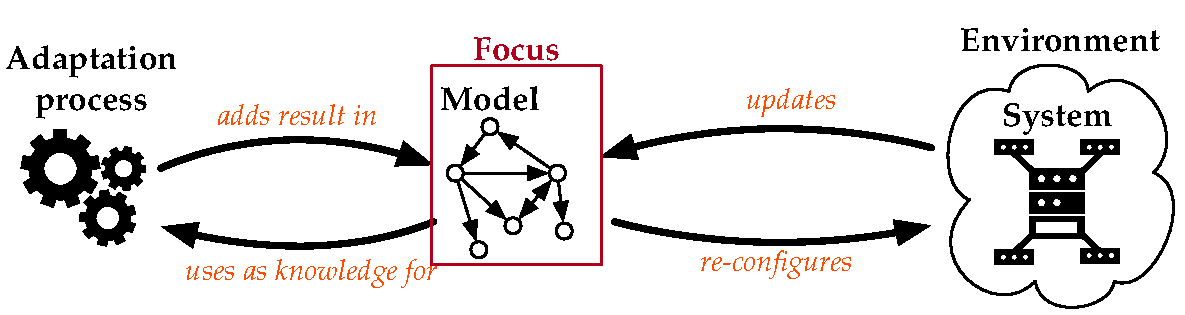
\includegraphics[width=.9\linewidth]{img/chapt-intro/context/mart-focus}
	\caption{Overview of the \gls{m@rt} and focus of the thesis}
	\label{fig:intro:context:m@rt}
\end{figure}
